%!TEX root = ../dokumentation.tex

\RequirePackage[l2tabu, orthodox]{nag}	% weist in Commandozeile bzw. log auf veraltete LaTeX Syntax hin

\documentclass[%
    pdftex,
    oneside,			% Einseitiger Druck.
    12pt,				% Schriftgroesse
    parskip=half,		% Halbe Zeile Abstand zwischen Absätzen.
    %topmargin = 10pt,	% Abstand Seitenrand (Std:1in) zu Kopfzeile [laut log: unused]
    headheight = 33pt,	% Höhe der Kopfzeile
    %headsep = 30pt,	% Abstand zwischen Kopfzeile und Text Body  [laut log: unused]
    headsepline,		% Linie nach Kopfzeile.
    footsepline,		% Linie vor Fusszeile.
    %footheight = 16pt,	% Höhe der Fusszeile
    abstracton,		% Abstract Überschriften
    DIV=calc,		% Satzspiegel berechnen
    BCOR=8mm,		% Bindekorrektur links: 8mm
    headinclude=false,	% Kopfzeile nicht in den Satzspiegel einbeziehen
    footinclude=false,	% Fußzeile nicht in den Satzspiegel einbeziehen
    listof=totoc,		% Abbildungs-/ Tabellenverzeichnis im Inhaltsverzeichnis darstellen
    toc=bibliography,	% Literaturverzeichnis im Inhaltsverzeichnis darstellen
]{scrreprt}	% Koma-Script report-Klasse, fuer laengere Bachelorarbeiten alternativ auch: scrbook

% Einstellungen laden
\usepackage{xstring}
\usepackage{ifpdf}
\usepackage{ifluatex}

%Bildquelle
%\usepackage[ngerman]{babel}
\usepackage{varwidth}
\usepackage{graphicx}
%\usepackage{hyperref}

\newcommand*{\quelle}{%
	\footnotesize Quelle:
}



\usepackage{lastpage}
\usepackage{fancyhdr}
\newcommand{\einstellung}[1]{%
    \expandafter\newcommand\csname #1\endcsname{}
    \expandafter\newcommand\csname setze#1\endcsname[1]{\expandafter\renewcommand\csname#1\endcsname{##1}}
}
\newcommand{\langstr}[1]{\einstellung{lang#1}}

% Flag für die Selbstständigkeitserklärung, Default: true
\newif\ifselbsterkl
\selbsterklfalse

% Flag für das Wasserzeichen auf dem Deckblatt, default: false
\newif\ifwatermark
\watermarkfalse

% Flag für roten Vertraulichkeitspunkt, default: false
\newif\ifreddot
\reddotfalse

% Flag für gelben Vertraulichkeitspunkt, default: false
\newif\ifyellowdot
\yellowdotfalse

% Flag für das Unterschriftenblatt, default: false
\newif\ifunterschriftenblatt
\unterschriftenblattfalse

% Flag für Einfügen der Seitenzahl bei Verweis auf Kapitel/Abschnitt, default: false
\newif\ifrefWithPages
\refWithPagesfalse

% Flag für Einfügen der Abstracts in deutsch und englisch, default: false
\newif\ifbothabstracts
\bothabstractsfalse

% Flag für Einfügen des Abkürzungsverzeichnis
\newif\ifabkverz
\abkverzfalse

% Flag für Einfügen des Abbildungsverzeichnisses
\newif\ifabbverz
\abbverzfalse

% Flag für Einfügen des Formelverzeichnisses
\newif\ifformelverz
\formelverzfalse

% Flag für Einfügen des Formelgroessenverzeichnisses
\newif\ifformelgroeverz
\formelgroeverzfalse 

% Flag für Einfügen des Listingsverzeichnisses
\newif\iflistverz
\listverzfalse

% Flag für Einfügen des Tabellenverzeichnisses
\newif\iftableverz
\tableverzfalse

% Flag für Einfügen des Sperrvermerks
\newif\ifsperrvermerk
\sperrvermerkfalse

% Flag für Einfügen des Abstracts
\newif\ifabstract
\abstractfalse

% Flag für Anhang
\newif\ifappendix
\appendixfalse

% Flag für Literaturverzeichnis
\newif\ifliteratur
\literaturfalse

% Flag für Glossar
\newif\ifglossar
\glossarfalse

% Flag für Inhaltsverzeichnis
\newif\ifinhalt
\inhaltfalse

% Flag für Reviewer
\newif\ifreviewer
\reviewerfalse

\einstellung{martrikelnr}
\einstellung{titel}
\einstellung{kurs}
\einstellung{datumAnfang}
\einstellung{datumAbgabe}
\einstellung{firma}
\einstellung{firmenort}
\einstellung{abgabeort}
\einstellung{abschluss}
\einstellung{studiengang}
\einstellung{dhbw}
\einstellung{betreuer}
\einstellung{gutachter}
\einstellung{zeitraum}
\einstellung{arbeit}
\einstellung{autor}
\einstellung{sprache}
\einstellung{schriftart}
\einstellung{kapitelabstand}
\einstellung{spaltenabstand}
\einstellung{zeilenabstand}
\einstellung{zitierstil}
\einstellung{selbsterkl}
\einstellung{semester}
\einstellung{studienrichtung}
\einstellung{jahrgang}
\einstellung{abteilung}
\einstellung{standort}
 % verfügbare Einstellungen
%%%%%%%%%%%%%%%%%%%%%%%%%%%%%%%%%%%%%%%%%%%%%%%%%%%%%%%%%%%%%%%%%%%%%%%%%%%%%%%
%                                   Einstellungen
%
% Hier können alle relevanten Einstellungen für diese Arbeit gesetzt werden.
% Dazu gehören Angaben u.a. über den Autor sowie Formatierungen.
%
%
%%%%%%%%%%%%%%%%%%%%%%%%%%%%%%%%%%%%%%%%%%%%%%%%%%%%%%%%%%%%%%%%%%%%%%%%%%%%%%%


%%%%%%%%%%%%%%%%%%%%%%%%%%%%%%%%%%%% Sprache %%%%%%%%%%%%%%%%%%%%%%%%%%%%%%%%%%%
%% Aktuell sind Deutsch und Englisch unterstützt.
%% Es werden nicht nur alle vom Dokument erzeugten Texte in
%% der entsprechenden Sprache angezeigt, sondern auch weitere
%% Aspekte angepasst, wie z.B. die Anführungszeichen und
%% Datumsformate.
\setzesprache{de} % de oder en
%%%%%%%%%%%%%%%%%%%%%%%%%%%%%%%%%%%%%%%%%%%%%%%%%%%%%%%%%%%%%%%%%%%%%%%%%%%%%%%%

%%%%%%%%%%%%%%%%%%%%%%%%%%%%%%%%%%% Angaben  %%%%%%%%%%%%%%%%%%%%%%%%%%%%%%%%%%%
%% Die meisten der folgenden Daten werden auf dem
%% Deckblatt angezeigt, einige auch im weiteren Verlauf
%% des Dokuments.
\setzemartrikelnr{8773151}
\setzekurs{TEL22GR3}
\setzetitel{Das Wurzelortskurvenverfahren für digitale Regelkreise}
\setzedatumAnfang{}
\setzedatumAbgabe{}
\setzefirma{Robert Bosch GmbH}
\setzefirmenort{Feuerbach}
\setzeabgabeort{}
\setzeabschluss{}
\setzestudiengang{Elektrotechnik}
\setzedhbw{Stuttgart}
\setzebetreuer{Dr. Samuel Quenzer-Hohmuth}
\setzegutachter{}
\setzezeitraum{25.11.2024 - 01.02.2025}
\setzearbeit{Praktikum 2 Regelungstechnik}
\setzeautor{Jan Tepel}
\setzesemester{5}
\setzestudienrichtung{-todo-}
\setzejahrgang{-todo-}
\setzeabteilung{-todo-}
\setzestandort{-todo-}

\inhalttrue                 % auskommentieren oder ändern zu \inhaltfalse, falls kein Inhaltsverzeichnis eingefügt werden soll
%\unterschriftenblatttrue    % auskommentieren oder ändern zu \unterschriftenblattfalse, falls kein Unterschriftenblatt eingefügt werden soll
\selbsterklfalse             % auskommentieren oder ändern zu \selbsterklfalse, wenn keine Selbstständigkeitserklärung benötigt wird
%\sperrvermerktrue           % auskommentieren oder ändern zu \sperrvermerkfalse, wenn kein Sperrvermerk benötigt wird
%\abkverztrue                % auskommentieren oder ändern zu \abkverzfalse, wenn kein Abkürzungsverzeichnis benötigt wird
%\abbverztrue                % auskommentieren oder ändern zu \abbverzfalse, wenn kein Abbildungsverzeichnis benötigt wird
%\tableverztrue              % auskommentieren oder ändern zu \tableverzfalse, wenn kein Tabellenverzeichnis benötigt wird
%\listverztrue               % auskommentieren oder ändern zu \listverzfalse, wenn kein Listingsverzeichnis benötigt wird
%\formelverztrue             % auskommentieren oder ändern zu \formelverzfalse, wenn kein Formelverzeichnis benötigt wird
%\formelgroeverztrue			% auskommentieren oder ändern zu \formelgroeverzfalse, wenn kein Formelgrößenverzeichnis benötigt wird
%\abstracttrue               % auskommentieren oder ändern zu \abstractfalse, wenn kein Abstract gewünscht ist
%\bothabstractsfalse          % auskommentieren oder ändern zu \bothabstractsfalse, wenn nur der Abstract in der Hauptsprache eingefügt werden soll
%\appendixtrue               % auskommentieren oder ändern zu \appendixfalse, wenn kein Anhang gewünscht ist
%\literaturtrue              % auskommentieren oder ändern zu \literaturfalse, wenn kein Literaturverzeichnis gewünscht ist (\appendixtrue muss gesetzt sein!)
%\glossartrue                % auskommentieren oder ändern zu \glossarfalse, wenn kein Glossar gewünscht ist (\appendixtrue muss gesetzt sein!)
\watermarkfalse             % auskommentieren oder ändern zu \watermarktrue, wenn Wasserzeichen auf dem Titelblatt eingefügt werden soll

\refWithPagesfalse          % ändern zu \refWithPagestrue, wenn die Seitenzahl bei Verweisen auf Kapitel engefügt werden sollen

\reviewertrue				% auskommentiren oder ändern zu \reviewerfalse wenn kein Gutachter gesetzt werden muss

% Angabe des roten/gelben Punktes auf dem Titelblatt zur Kennzeichnung der Vertraulichkeitsstufe.
% Mögliche Angaben sind \yellowdottrue und \reddottrue. Werden beide angegeben, wird der rote Punkt gezeichnet.
% Wird keines der Kommandos angegeben, wird kein Punkt gezeichnet
\yellowdotfalse

%%%%%%%%%%%%%%%%%%%%%%%%%%%%%%%%%%%%%%%%%%%%%%%%%%%%%%%%%%%%%%%%%%%%%%%%%%%%%%%%

%%%%%%%%%%%%%%%%%%%%%%%%%%%% Literaturverzeichnis %%%%%%%%%%%%%%%%%%%%%%%%%%%%%%
%% Bei Fehlern während der Verarbeitung bitte in ads/header.tex bei der
%% Einbindung des Pakets biblatex (ungefähr ab Zeile 110,
%% einmal für jede Sprache), biber in bibtex ändern.
\newcommand{\ladeliteratur}{%
	\addbibresource{bibliographie.bib}
	%\addbibresource{weitereDatei.bib}
}

%% Zitierstil
%% siehe: http://ctan.mirrorcatalogs.com/macros/latex/contrib/biblatex/doc/biblatex.pdf (3.3.1 Citation Styles)
%% mögliche Werte z.B numeric-comp, alphabetic, authoryear
\setzezitierstil{alphabetic}
%%%%%%%%%%%%%%%%%%%%%%%%%%%%%%%%%%%%%%%%%%%%%%%%%%%%%%%%%%%%%%%%%%%%%%%%%%%%%%%%

%%%%%%%%%%%%%%%%%%%%%%%%%%%%%%%%% Layout %%%%%%%%%%%%%%%%%%%%%%%%%%%%%%%%%%%%%%%
%% Verschiedene Schriftarten
% laut nag Warnung: palatino obsolete, use mathpazo, helvet (option scaled=.95), courier instead
\setzeschriftart{lmodern} % palatino oder goudysans, lmodern, libertine

%% Abstand vor Kapitelüberschriften zum oberen Seitenrand
\setzekapitelabstand{20pt}

%% Spaltenabstand
\setzespaltenabstand{10pt}
%%Zeilenabstand innerhalb einer Tabelle
\setzezeilenabstand{1.5}
%%%%%%%%%%%%%%%%%%%%%%%%%%%%%%%%%%%%%%%%%%%%%%%%%%%%%%%%%%%%%%%%%%%%%%%%%%%%%%%% % lese Einstellungen

\newcommand{\iflang}[2]{%
  \IfStrEq{\sprache}{#1}{#2}{}
}

\langstr{abkverz}
\langstr{anhang}
\langstr{glossar}
\langstr{deckblattabschlusshinleitung}
\langstr{artikelstudiengang}
\langstr{studiengang}
\langstr{anderdh}
\langstr{von}
\langstr{dbbearbeitungszeit}
\langstr{dbmatriknr}
\langstr{dbkurs}
\langstr{dbfirma}
\langstr{dbbetreuer}
\langstr{dbgutachter}
\langstr{sperrvermerk}
\langstr{erklaerung}
\langstr{abstract}
\langstr{listingname}
\langstr{listlistingname}
\langstr{listingautorefname}
\langstr{selbsterkl}
\langstr{formelsammlung}
\langstr{kopfz}
\langstr{fussz}
\langstr{seite}
\langstr{seitevon}
\langstr{stand}
\langstr{formelgroeverz} % verfügbare Strings
\input{lang/\sprache} % Übersetzung einlesen


%\lstset{language=Matlab}
\newcommand{\citem}[1]{\item[\texttt{#1}]} % Code-Item für description-Liste
%\newcommand\todo[1]{\textit{\textcolor{red}{TODO: #1}}\message{LaTeX Warning: \noexpand TODO item left in line \the\inputlineno}} % Todo-Item
\newcommand\todo[1]{\textit{\textcolor{red}{TODO: #1}}} % Todo-Item
\usepackage{pdfpages}         % pdf-Seiten einbinden

%% Farben (Angabe in HTML-Notation mit großen Buchstaben)
\newcommand{\ladefarben}{%
	\definecolor{LinkColor}{HTML}{00007A}
	\definecolor{ListingBackground}{HTML}{FCF7DE}
}
%% Mathematikpakete benutzen (Pakete aktivieren)
%\usepackage{amsmath}
%\usepackage{amssymb}

%% Programmiersprachen Highlighting (Listings)
\newcommand{\listingsettings}{%
	\lstset{%
		language=C++,			% Standardsprache des Quellcodes
		%numbers=left,			% Zeilennummern links
		%stepnumber=1,			% Jede Zeile nummerieren.
		%numbersep=5pt,			% 5pt Abstand zum Quellcode
		%numberstyle=\tiny,		% Zeichengrösse 'tiny' für die Nummern.
		breaklines=true,		% Zeilen umbrechen wenn notwendig.
		breakautoindent=true,	% Nach dem Zeilenumbruch Zeile einrücken.
		postbreak=\space,		% Bei Leerzeichen umbrechen.
		tabsize=2,				% Tabulatorgrösse 2
		basicstyle=\ttfamily\footnotesize, % Nichtproportionale Schrift, klein für den Quellcode
		showspaces=false,		% Leerzeichen nicht anzeigen.
		showstringspaces=false,	% Leerzeichen auch in Strings ('') nicht anzeigen.
		extendedchars=true,		% Alle Zeichen vom Latin1 Zeichensatz anzeigen.
		captionpos=b,			% sets the caption-position to bottom
		%backgroundcolor=\color{ListingBackground}, % Hintergrundfarbe des Quellcodes setzen.
		numbers=left,
		numberstyle=\tiny,
		xleftmargin=0pt,		% Rand links
		xrightmargin=0pt,		% Rand rechts
		frame=single,			% Rahmen an
		frameround=ffff,
		rulecolor=\color{darkgray},	% Rahmenfarbe
		%fillcolor=\color{ListingBackground},
		keywordstyle=\color[rgb]{0.133,0.133,0.6},
		commentstyle=\color[rgb]{0.133,0.545,0.133},
		stringstyle=\color[rgb]{0.627,0.126,0.941},
    aboveskip=1.5em,
	}
}





%%%%%%%%%%%%%%%%%%%%%%%%%%%%% Kopf-/Fußzeilenwechsel %%%%%%%%%%%%%%%%%%%%%%%%%%%
\setlength{\headheight}{40pt}

\newcommand{\setpagestylehead}{%
    \fancypagestyle{plain}{%
        \fancyhf{}
        \fancyhead[L]{\vspace{0.5cm}\small \langkopfz}
        \fancyhead[R]{
            \hspace{2.0cm}
            %trim=left bottom right top
            \iflang{de}{
				\begin{textblock*}{188mm}(-5mm,3mm)            	
            	
\includegraphics[height=2cm]{images/dhbw_de}
            	\end{textblock*}
            	}
            \iflang{en}{
            	\begin{textblock*}{188mm}(-5mm,3mm)            	
            	
\includegraphics[height=1.8cm]{images/dhbw_en}
            	\end{textblock*}
            	}
            \iflang{de}{
				\begin{textblock*}{188mm}(0mm,0mm)            	
            	%
\includegraphics[height=2.7cm]{images/Bosch_Logo_Kopfzeile}
            	\end{textblock*}
            	}
            \iflang{en}{
            	\begin{textblock*}{188mm}(0mm,0mm)            	
            	%
\includegraphics[height=2.2cm]{images/Bosch_Logo_Kopfzeile_en}
            	\end{textblock*}
            	}
        }
        \fancyfoot[L]{
            \noindent{\tiny \langfussz\\
                \begin{tabular*}{16cm}{@{\extracolsep{\fill}}l>{\raggedleft}p{8cm}}
                    {\tiny \langstand: \today} & 
                    {\tiny \langseite\ \thepage\ \langseitevon\ \pageref*{endOfRomanNumbering}\vspace{1cm}}\tabularnewline
                \end{tabular*}
            }
        }
    }
    \pagestyle{plain}
    \pagenumbering{roman}
}    

\newcommand{\setpagestylecontent}{
\fancypagestyle{plain}{%
        \fancyhf{}
        \fancyhead[L]{\vspace{0.5cm}\small \langkopfz}
        \fancyhead[R]{
            \hspace{2.0cm}
            %trim=left bottom right top
            \iflang{de}{
            	\begin{textblock*}{188mm}(-5mm,3mm)            	
            	
\includegraphics[height=2cm]{images/dhbw_de}
            	\end{textblock*}
            	}
            \iflang{en}{
            	\begin{textblock*}{188mm}(-5mm,3mm)            	
            	
\includegraphics[height=1.8cm]{images/dhbw_en}
            	\end{textblock*}
            	}
            \iflang{de}{
				\begin{textblock*}{188mm}(0mm,0mm)            	
            	%
\includegraphics[height=2.7cm]{images/Bosch_Logo_Kopfzeile}
            	\end{textblock*}
            	}
            \iflang{en}{
            	\begin{textblock*}{188mm}(0mm,0mm)            	
            	%
\includegraphics[height=2.2cm]{images/Bosch_Logo_Kopfzeile_en}
            	\end{textblock*}
            	}
        }
        \fancyfoot[L]{
            \noindent{\tiny \langfussz\\
                \begin{tabular*}{16cm}{@{\extracolsep{\fill}}l>{\raggedleft}p{8cm}}
                    {\tiny \langstand: \today} & 
                    {\tiny \langseite\ \thepage\ \langseitevon\ \pageref*{endOfArabicNumbering}\vspace{1cm}}\tabularnewline
                \end{tabular*}
            }
        }
    }
    \pagestyle{plain}
    \pagenumbering{arabic}
}

\newcommand{\setpagestylefoot}{
\fancypagestyle{plain}{%
        \fancyhf{}
        \fancyhead[L]{\vspace{0.5cm}\small \langkopfz}
        \fancyhead[R]{
            \hspace{2.0cm}
            %trim=left bottom right top
            \iflang{de}{
				\begin{textblock*}{188mm}(-5mm,3mm)            	
            	
\includegraphics[height=2cm]{images/dhbw_de}
            	\end{textblock*}
            	}
            \iflang{en}{
            	\begin{textblock*}{188mm}(-34mm,7mm)            	
            	
\includegraphics[height=1.2cm]{images/dhbw_en}
            	\end{textblock*}
            	}
            \iflang{de}{
				\begin{textblock*}{188mm}(0mm,0mm)            	
            	%
\includegraphics[height=2.7cm]{images/Bosch_Logo_Kopfzeile}
            	\end{textblock*}
            	}
            \iflang{en}{
            	\begin{textblock*}{188mm}(0mm,0mm)            	
            	%
\includegraphics[height=2.2cm]{images/Bosch_Logo_Kopfzeile_en}
            	\end{textblock*}
            	}
        }
        \fancyfoot[L]{
            \noindent{\tiny \langfussz\\
                \begin{tabular*}{16cm}{@{\extracolsep{\fill}}l>{\raggedleft}p{8cm}}
                    {\tiny \langstand: \today} & 
                    {\tiny \langseite\ \thepage\ \langseitevon\ \pageref*{LastPage}\vspace{1cm}}\tabularnewline
                \end{tabular*}
            }
        }
    }
    \pagestyle{plain}
    \pagenumbering{Alph}
}


%%%%%%%%%%%%%%%%%%%%%%%%%%%%%%%%%%%%%%%%%%%%%%%%%%%%%%%%%%%%%%%%%%%%%%%%%%%%%%%%

% Einstellung der Sprache des Paketes Babel und der Verzeichnisüberschriften

\iflang{de}{
	\usepackage[english, ngerman]{babel}
	\selectlanguage{ngerman}
}
\iflang{en}{
	\usepackage[ngerman, english]{babel}
	\selectlanguage{english}
}

\usepackage{amssymb}
\usepackage[utf8]{inputenc}
\usepackage[T1]{fontenc}
\usepackage{tikz}
\usepackage{xcolor}
\usepackage{additionalPackages/tikz-uml} % UML Diagramme
\usepackage[european]{additionalPackages/circuitikz}
%%%%%%% Package Includes %%%%%%%

\usepackage[margin=2.5cm,foot=1cm,top=3cm,bottom=3cm]{geometry}	% Seitenränder und Abstände
\usepackage[activate]{microtype} %Zeilenumbruch und mehr
\usepackage[onehalfspacing]{setspace}
\usepackage{makeidx}
\usepackage[autostyle=true,german=quotes]{csquotes}
\usepackage{longtable}
\usepackage{enumitem}	% mehr Optionen bei Aufzählungen
\usepackage{graphicx}
\usepackage{xcolor} 	% für HTML-Notation
\usepackage{float}
\usepackage{array}
\usepackage{calc}		% zum Rechnen (Bildtabelle in Deckblatt)
\usepackage[right]{eurosym}
\usepackage{wrapfig}
\usepackage{pgffor} % für automatische Kapiteldateieinbindung
\usepackage[perpage, hang, multiple, stable]{footmisc} % Fussnoten
\usepackage{acronym}
\usepackage[absolute]{textpos}
%\usepackage[printonlyused, footnote]{acronym} % falls gewünscht kann die Option footnote eingefügt werden, dann wird die Erklärung nicht inline sondern in einer Fußnote dargestellt
\usepackage{scrhack} % in Kombination mit listings-Package kommt es zu Warnings, dieses Paket verhindert die Warnings! Ggf. auskommentieren und die Warnings akzeptieren falls Verzeichnisse nicht so dargestellt werden wie gewünscht
\usepackage{listings} % Code-Listings
%\usepackage[numbered, framed]{matlab-prettifier}
\usepackage[framed]{matlab-prettifier} % .sty-Datei muss vorhanden sein! Kann auskommentiert werden, falls keine Matlab-Listings in der Arbeit enthalten sind.
\usepackage{color, colortbl}  %Für Highlighten der Tabellenzeilen
\usepackage{amsmath}% http://ctan.org/pkg/amsmath


% eine Kommentarumgebung "k" (Handhabe mit \begin{k}<Kommentartext>\end{k},
% Kommentare werden rot gedruckt). Wird \% vor excludecomment{k} entfernt,
% werden keine Kommentare mehr gedruckt.
\usepackage{comment}
\specialcomment{k}{\begingroup\color{red}}{\endgroup}
%\excludecomment{k}


%%%%%% Configuration %%%%%

%% Anwenden der Einstellungen

\usepackage{\schriftart}
\ladefarben{}

% Titel, Autor und Datum
\title{\titel}
\author{\autor}
\date{\datum}

%\usepackage[list=true]{subcaption}

% PDF Einstellungen
\usepackage[%
pdftitle={\titel},
pdfauthor={\autor},
pdfsubject={\arbeit},
pdfcreator={pdflatex, LaTeX with KOMA-Script},
pdfpagemode=UseOutlines, 		% Beim Oeffnen Inhaltsverzeichnis anzeigen
pdfdisplaydoctitle=true, 		% Dokumenttitel statt Dateiname anzeigen.
pdflang={\sprache} 			% Sprache des Dokuments.
]{hyperref}

% (Farb-)einstellungen für die Links im PDF
\hypersetup{%
    colorlinks=true, 		% Aktivieren von farbigen Links im Dokument
    linkcolor=black, 	    % Farbe festlegen
    citecolor=LinkColor,
    filecolor=LinkColor,
    menucolor=LinkColor,
    urlcolor=LinkColor,
    %linktocpage=true, 		% Nicht der Text sondern die Seitenzahlen in Verzeichnissen klickbar
    linktoc=all,            % Seitenzahlen und Text klickbar
    bookmarksnumbered=true 	% Überschriftsnummerierung im PDF Inhalt anzeigen.
}
% Workaround um Fehler in Hyperref, muss hier stehen bleiben
\usepackage{bookmark} %nur ein latex-Durchlauf für die Aktualisierung von Verzeichnissen nötig

% Schriftart in Captions etwas kleiner
\addtokomafont{caption}{\small}

\usepackage{subfig}

% Literaturverweise (sowohl deutsch als auch englisch)
\iflang{de}{%
\usepackage[
    backend=bibtex,		% empfohlen. Falls biber Probleme macht: bibtex
    bibwarn=true,
    bibencoding=utf8,	% wenn .bib in utf8, sonst ascii
    sortlocale=de_DE,
    style=\zitierstil,
]{biblatex}
}
\iflang{en}{%
\usepackage[
    backend=bibtex,		% empfohlen. Falls biber Probleme macht: bibtex
    bibwarn=true,
    bibencoding=utf8,	% wenn .bib in utf8, sonst ascii
    sortlocale=en_US,
    style=\zitierstil,
]{biblatex}
}


\ladeliteratur{}
%\bibliography{bibliographie}

% Glossar
\usepackage[nonumberlist,toc]{glossaries}
\usepackage{blindtext} % Blindtext-Package. Common Usage: \blindtext für einzelnen Abschnitt, \Blindtext für mehrere Abschnitte

%%%%%% Additional settings %%%%%%

% Hurenkinder und Schusterjungen verhindern
% http://projekte.dante.de/DanteFAQ/Silbentrennung
\clubpenalty = 10000 % schließt Schusterjungen aus (Seitenumbruch nach der ersten Zeile eines neuen Absatzes)
\widowpenalty = 10000 % schließt Hurenkinder aus (die letzte Zeile eines Absatzes steht auf einer neuen Seite)
\displaywidowpenalty=10000

\setcounter{biburlnumpenalty}{100}
\setcounter{biburlucpenalty}{100}
\setcounter{biburllcpenalty}{100}

% Bildpfad
\graphicspath{{images/}}

% Einige häufig verwendete Sprachen
\lstloadlanguages{PHP,Python,Java,C,C++,bash}
\listingsettings{}
% Umbennung des Listings
\renewcommand\lstlistingname{\langlistingname}
\renewcommand\lstlistlistingname{\langlistlistingname}
\def\lstlistingautorefname{\langlistingautorefname}

% Abstände in Tabellen
\setlength{\tabcolsep}{\spaltenabstand}
\renewcommand{\arraystretch}{\zeilenabstand}

\usepackage{xspace}
\newcommand{\lastcontentpage}{}
\usepackage{amsfonts}

\usetikzlibrary{shapes,arrows,calc}
\usepackage{relsize}

\usepackage{censor}

\usepackage{eso-pic}


%% Paket um Textteile drehen zu können
%\usepackage{rotating}
%% Paket um Seite im Querformat anzuzeigen
%\usepackage{lscape}

\newcommand\Watermark{%
    \put(0,0){%
        \parbox[b][\paperheight]{\paperwidth}{%
            \vfill
            
\includepdf[scale=0.8,angle=50,pages={1},pagecommand={}]{ads/watermark}
            \vfill
        }
    }
}

\ifrefWithPages
    %RJG8FE: add a pageref to autoref whenever the referenced page is not the same as the current one
    %        useful for printed documents without clickable hyperlinks
    \AtBeginDocument{\let\oldautoref\autoref}
    \AtBeginDocument{
        \renewcommand{\autoref}[1]{%
            \oldautoref{#1}%
            \ifthenelse{\thepage=\pageref{#1}}% if current page number equals the referenced page number
            {}% then add nothing
            { (S. \pageref{#1})}% else add the text
        }
    }
\fi

\usepackage{amssymb} % Erweiterung der Symbole in Mathematikumgebung

\iflang{de}{\usepackage{icomma}} % Europäsiches Komma in Formeln
\DeclareNewTOC[%
 forcenames,
 type=formel,
 name={Formel},%
 listname={\langformelsammlung}
]{for}

\iflang{de}{%
    \newcommand*{\formelentry}[1]{%
     \addcontentsline{for}{formel}{\protect\numberline{\theequation} #1}%
    }
}
\iflang{en}{%
    \newcommand*{\formelentry}[1]{%
     \addcontentsline{for}{formel}{\protect\numberline{\theequation} #1}%
    }
}
\makeglossaries
%!TEX root = ../dokumentation.tex

%
% vorher in Konsole folgendes aufrufen:
%	makeglossaries makeglossaries dokumentation.acn && makeglossaries dokumentation.glo
%
% oder makeglossaries dokumentation
%
% Um das auszuführen, braucht man ActivePerl oder ein ähnliches Programm. ActivePerl kann man bei MyIT Services beantragen

%
% Glossareintraege --> referenz, name, beschreibung
% Aufruf mit \gls{...}
%
% Glossar wird nur angezeigt, wenn Glossareintrag in Text referenziert wird
%
\newglossaryentry{Glossareintrag}{name={Glossareintrag},plural={Glossareinträge},description={Ein Glossar beschreibt verschiedenste Dinge in kurzen Worten}}

\newglossaryentry{ct}{name={Compiletime},description={Die Compiletime ist der Zeitpunkt, zu dem ein Programm vom Compiler in vom Computer ausführbaren Maschinencode übersetzt wird}}

\newglossaryentry{rt}{name={Runtime},description={Die Runtime ist der Zeitpunkt, zu dem ein bereits in Maschinencode übersetztes Programm vom Benutzer ausgeführt wird}}

\begin{document}
    \StopCensoring

    % Wasserzeichen einfügen, falls Flag gesetzt
    \ifwatermark
        \AddToShipoutPicture{\Watermark}
    \fi
    \setpagestylehead
    % Deckblatt
    \begin{spacing}{1}
        %!TEX root = ../dokumentation.tex

\begin{titlepage}
	\begin{longtable}{p{8.2cm} p{5.4cm}}
		{
			\raisebox{\ht\strutbox-\totalheight}{
				\iflang{de}{
					%trim=left bottom right top
					%\includegraphics[width=7cm,trim=1.3cm 0 -1.3cm -0.5cm]{Bosch_Logo_DE}
				}
				\iflang{en}{
					%\includegraphics[width=7cm,trim=1.3cm 0 -1.3cm -0.5cm]{Bosch_Logo_EN}
				}
			}
		} &
		{
			\raisebox{\ht\strutbox-\totalheight}{
				\iflang{de}{
\includegraphics[height=2.5cm]{dhbw_de}}
				\iflang{en}{
\includegraphics[height=2.5cm]{dhbw_en}}
			}
		}
	\end{longtable}
	
	
	%\iflang{de}
	%{
	%	\begin{textblock*}{188mm}(0mm,23mm)
	%	
\includegraphics[width=88mm]{Bosch_Logo_Titelblatt}
	%	\end{textblock*}
	%}
	
	%\iflang{en}
	%{
%		\begin{textblock*}{188mm}(0mm,21mm)
%			
\includegraphics[width=95mm]{Bosch_Logo_Titelblatt_en}
%		\end{textblock*}
	%}
	
	\enlargethispage{20mm}
	\begin{center}
		\begin{doublespace}
			\vspace*{12mm}	{\LARGE\textbf \titel }\\
			\vspace*{5mm}
		\end{doublespace}
		
		\begin{tikzpicture}		
		\ifreddot
		\tikz\draw[fill=red,draw=red](-4,2) circle (1.4cm);
		\else
		\ifyellowdot
		\tikz\draw[fill=yellow,draw=yellow](-4,2) circle (1.4cm);
		\else
		%\tikz\draw[fill=green,draw=green](-4,1) circle (1.4cm);
		\fi
		\fi
		\end{tikzpicture}
		\vspace{-1.4cm}
		\\
		
		\vspace*{12mm}	{\large\textbf \arbeit }\\
		
		%	\vspace*{12mm}	\langdeckblattabschlusshinleitung\\
		\vspace*{3mm}		{\textbf \abschluss}\\
		\vspace*{12mm}	\langartikelstudiengang{} \langstudiengang{} \studiengang\\
		\vspace*{3mm}		\langanderdh{} \dhbw\\
		\vspace*{12mm}	\langvon\\
		\vspace*{3mm}		{\large\textbf \autor}\\
		\vspace*{12mm}	\datumAbgabe
	\end{center}
	\vfill
	\begin{spacing}{1.2}
		\begin{tabbing}
			mmmmmmmmmmmmmmmmmmmmmmmmmm             \= \kill
			\textbf{\langdbbearbeitungszeit}       \>  \zeitraum\\
			\textbf{\langdbmatriknr, \langdbkurs}  \>  \martrikelnr, \kurs\\
			%\textbf{\langdbfirma}                  \>  \firma, \firmenort\\
			\textbf{\langdbbetreuer}               \>  \betreuer\\
			\ifreviewer
			%\textbf{\langdbgutachter}              \>  \gutachter\\
			\fi
		\end{tabbing}
	\end{spacing}
\end{titlepage}

    \end{spacing}
    
    \newpage
    \ifwatermark
        \ClearShipoutPicture
    \fi
    \pagenumbering{Roman}
    \ifunterschriftenblatt
        %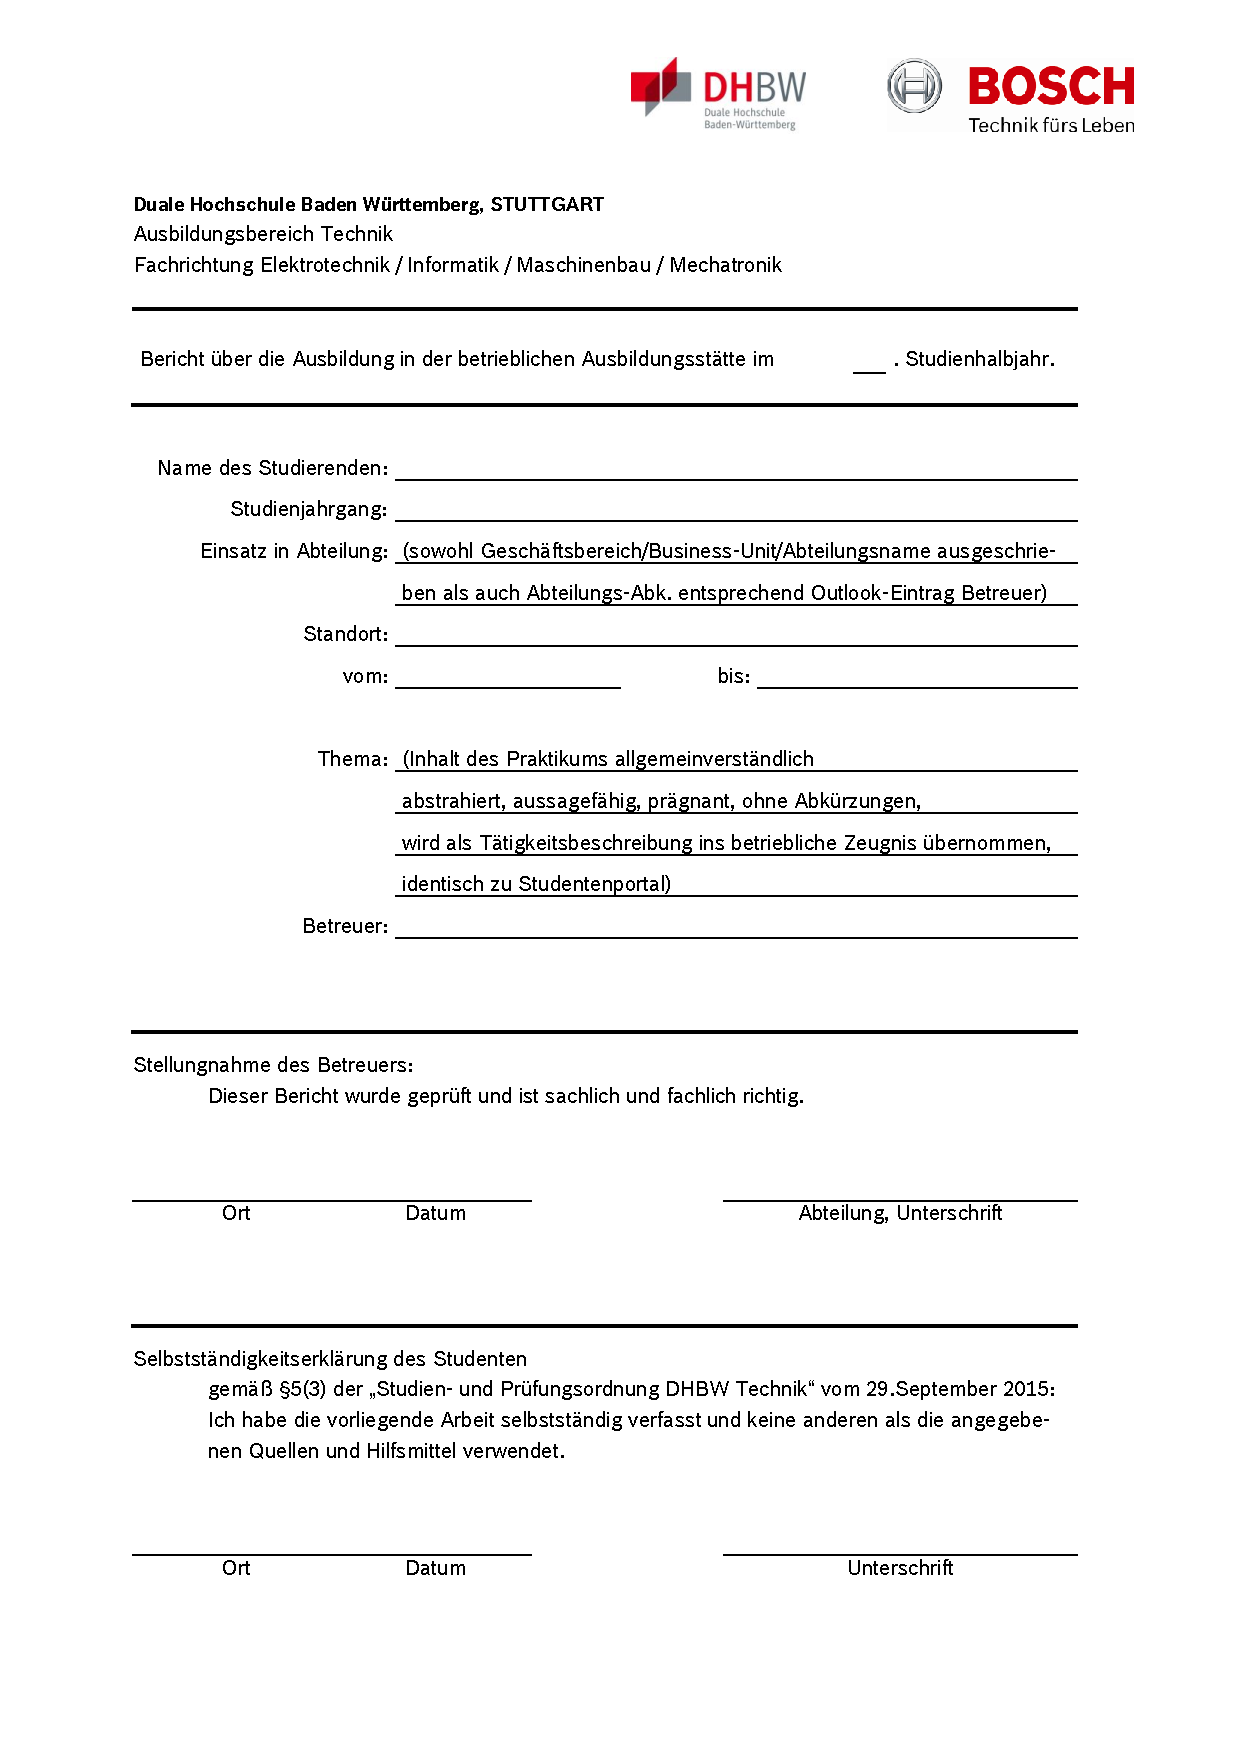
\includepdf[scale=1,clip,trim=0cm 1.5cm 0cm 2.5cm,pages={1},pagecommand={}]{ads/unterschriftenblatt}
        %!TEX root = ../dokumentation.tex
\thispagestyle{plain}

{\footnotesize Duale Hochschule Baden-Württemberg, Stuttgart }{\footnotesize \par}

{\footnotesize Ausbildungsbereich Technik, Fachrichtung \studienrichtung }{\footnotesize \par}

{\footnotesize \rule[0.5ex]{1\columnwidth}{1pt}}{\footnotesize \par}

{\footnotesize 	Bericht über die Ausbildung in der betrieblichen Ausbildungsstätte im }%
\begin{tabular}{c}
{\footnotesize \semester}\tabularnewline
\hline 
\end{tabular}{\footnotesize . Studienhalbjahr.}{\footnotesize \par}

{\footnotesize \rule[0.5ex]{1\columnwidth}{1pt}}{\footnotesize \par}

{\footnotesize }%
\begin{tabular*}{16cm}{@{\extracolsep{\fill}}>{\raggedleft}p{4cm}>{\centering}p{4cm}cc}
{\footnotesize Name des Studierenden:} & \multicolumn{3}{l}{\footnotesize \autor}\tabularnewline
\cline{2-4} 
{\footnotesize Studienjahrgang:} & \multicolumn{3}{>{\raggedright}p{11cm}}{\footnotesize \jahrgang}\tabularnewline
\cline{2-4} 
{\footnotesize Einsatz in Abteilung:} & \multicolumn{3}{>{\raggedright}p{11cm}}{\footnotesize \abteilung}\tabularnewline
\cline{2-4} 
{\footnotesize Standort:} & \multicolumn{3}{>{\raggedright}p{11cm}}{\footnotesize \standort}\tabularnewline
\cline{2-4} 
{\footnotesize Thema:} & \multicolumn{3}{>{\raggedright}p{11cm}}{\footnotesize \titel}\tabularnewline
\cline{2-4} 
{\footnotesize Betreuer:} & \multicolumn{3}{>{\raggedright}p{11cm}}{\footnotesize \betreuer}\tabularnewline
\cline{2-4} 
{\footnotesize vom:} & {\footnotesize \datumAnfang} & {\footnotesize bis:} & {\footnotesize \datumAbgabe}\tabularnewline
\cline{2-2} \cline{4-4} 
\end{tabular*}{\footnotesize \par}

{\footnotesize \vspace{3mm}
}{\footnotesize \par}

{\footnotesize \rule[0.5ex]{1\columnwidth}{1pt}}{\footnotesize \par}

{\footnotesize Stellungnahme des Betreuers:}{\footnotesize \par}

{\footnotesize \hspace{1cm}Dieser Bericht wurde geprüft und ist sachlich und fachlich richtig. }{\footnotesize \par}

{\footnotesize \vspace{1cm}
}{\footnotesize \par}

{\footnotesize }%
\begin{tabular*}{16cm}{@{\extracolsep{\fill}}>{\centering}p{2cm}>{\centering}p{2cm}c>{\centering}p{6cm}}
\cline{1-2} \cline{4-4} 
{\footnotesize Ort} & {\footnotesize Datum} & ~ & {\footnotesize Abteilung, Unterschrift}\tabularnewline
\end{tabular*}{\footnotesize{} }{\footnotesize \par}

{\footnotesize \rule[0.5ex]{1\columnwidth}{1pt}}\\
{\footnotesize Selbstständigkeitserklärung des Studenten }{\footnotesize \par}

\begin{tabular*}{16cm}{@{\extracolsep{\fill}}>{\centering}p{1mm}p{15cm}}
 & {\footnotesize Gemäß \S5(2) der "`Studien- und Prüfungsordnung DHBW Technik"' vom 29. September 2015: Ich habe die vorliegende Arbeit selbstständig verfasst und keine anderen als die angegebenen Quellen und Hilfsmittel verwendet.
}\tabularnewline
\end{tabular*}

{\footnotesize \vspace{1cm}
}{\footnotesize \par}

{\footnotesize }%
\begin{tabular*}{16cm}{@{\extracolsep{\fill}}>{\centering}p{2cm}>{\centering}p{2cm}c>{\centering}p{6cm}}
\cline{1-2} \cline{4-4} 
{\footnotesize Ort} & {\footnotesize Datum} & ~ & {\footnotesize Unterschrift}\tabularnewline
\end{tabular*}{\footnotesize{}  }{\footnotesize \par}

        \newpage
    \fi
    
    % Sperrvermerk
    \ifsperrvermerk
    %!TEX root = ../dokumentation.tex

\thispagestyle{plain}
% Sperrvermerk direkt hinter Titelseite
\section*{\\\langsperrvermerk}

\vspace*{2em}

\iflang{de}{%
  Die vorliegende {\arbeit} mit dem Titel \begin{center}{\itshape{}\titel{}\/}\end{center}  enthält unternehmensinterne bzw. vertrauliche Informationen der {\firma}, ist deshalb mit einem Sperrvermerk versehen und wird ausschließlich zu Prüfungszwecken am Studiengang {\studiengang} der Dualen Hochschule Baden-Württemberg {\dhbw} vorgelegt. 
	\\
	\\
	Der Inhalt dieser Arbeit darf weder als Ganzes noch in Auszügen Personen außerhalb des Prüfungsprozesses und des Evaluationsverfahrens zugänglich gemacht werden, sofern keine anders lautende Genehmigung der Ausbildungsstätte ({\firma}) vorliegt.
}

%http://www.ib.dhbw-mannheim.de/fileadmin/ms/bwl-ib/Downloads_alt/Leitfaden_31.05.pdf

\iflang{en}{%
  The {\arbeit} on hand 
  \begin{center}{\itshape{} \titel{}\/}\end{center} 
   contains internal respective confidential data of {\firma}. It is intended solely for inspection by the assigned examiner, the head of the {\studiengang} department and, if necessary, the Audit Committee \langanderdh{} {\dhbw}. It is strictly forbidden:
    \begin{itemize}
    \item to distribute the content of this paper (including data, figures, tables, charts etc.) as a whole or in extracts,
    \item to make copies or transcripts of this paper or of parts of it,
    \item to display this paper or make it available in digital, electronic or virtual form.
    \end{itemize}
  Exceptional cases may be considered through permission granted in written form by the author and {\firma}.
}

\vspace{3em}

\abgabeort, \datumAbgabe
\vspace{4em}

\rule{6cm}{0.4pt}\\
\autor

    \newpage
    \fi

    % Selbstständigkeitserklärung nur einfügen, wenn Flag in den Einstellungen gesetzt ist
    \ifselbsterkl
        %!TEX root = ../dokumentation.tex

\thispagestyle{plain}
% Sperrvermerk direkt nach Selbstständigkeitserklärung
\section*{Selbstständigkeitserklärung}
%\section*{\\\langselbsterkl}

\vspace*{2em}


Wir versichern hiermit, dass wir unsere {\arbeit} mit dem Thema: {\itshape{} \titel{}\/} selbstständig verfasst und keine anderen als die angegebenen Quellen und Hilfsmittel benutzt habe.

\vspace{3em}

Stuttgart, \datumAbgabe
\vspace{4em}

\rule{6cm}{0.4pt} \hspace{3.8cm}  \rule{6cm}{0.4pt}\\
Lukas Mack \hspace{7.55cm} Jan Tepel

        \newpage
    \fi

    % Abstract
    \ifabstract
        %!TEX root = ../dokumentation.tex


\newcommand{\deAbstractContent}{
Diese Studienarbeit befasst sich mit der Integration einer Brennstoffzelle als Reichweitenextender in das Solo Electra 720. Der Schwerpunkt des bearbeiteten Teilprojekts lag auf der Inbetriebnahme der Brennstoffzelle und der Herstellung einer funktionierenden Schnittstelle zwischen Brennstoffzelle und Software. Aufgrund fehlenden Zugangs zu Wasserstoff wurde die Brennstoffzelle leider nicht unter realen Bedingungen getestet; stattdessen wurde die Kommunikation und Steuerung über einen Laptop erfolgreich eingerichtet.

Theoretische Grundlagen zu den Themen Elektromobilität, Wasserstoff als Energieträger, und die Funktion von Protonenaustauschmembran-Brennstoffzellen (PEMFC) bilden die Basis dieser Arbeit.

Das praktische Ergebnis zeigt, dass die Verbindung zwischen Brennstoffzelle und Software zuverlässig umgesetzt werden konnte. Dies legt eine Grundlage für künftige Projekte, die auf den Ausbau und Testbetrieb eines wasserstoffbetriebenen Systems abzielen.
}

\newcommand{\enAbstractContent}{
This study focuses on integrating a fuel cell as a range extender into the Solo Electra 720. The primary goal of the project was to commission the fuel cell and establish a functioning interface between the fuel cell and software. Due to the lack of access to hydrogen, the fuel cell was not tested under real operating conditions; instead, successful communication and control were established via a laptop.

Theoretical foundations on topics such as electromobility, hydrogen as an energy carrier, and the basics of proton exchange membrane fuel cells (PEMFC) underpin this work.

The practical results demonstrate that the connection between the fuel cell and the software was successfully implemented. This serves as a foundation for future projects focused on expanding and testing hydrogen-powered systems.
}

%%%%%%%% Ab hier nicht mehr anfassen! %%%%%%%%

\newcommand{\deAbstract}{%
    \renewcommand{\abstractname}{Kurzfassung} % Text für Überschrift
    \begin{abstract}
        \thispagestyle{plain}
        \deAbstractContent
    \end{abstract}
}

\newcommand{\enAbstract}{
    \renewcommand{\abstractname}{\langabstract} % Text für Überschrift
    \begin{abstract}
        \thispagestyle{plain}
        \enAbstractContent
    \end{abstract}
}

\iflang{de}{
    \deAbstract
    \ifbothabstracts
        \clearpage
      %  \begin{otherlanguage}{english}
            \enAbstract
     %   \end{otherlanguage}
    \fi
}

\iflang{en}{
    \enAbstract
    \ifbothabstracts
        \clearpage
        \begin{otherlanguage}{ngerman}
            \deAbstract
        \end{otherlanguage}
    \fi
}
        \newpage
    \fi

    \pagestyle{plain}		% nur Seitenzahlen im Fuß

    %\RedeclareSectionCommand[beforeskip=\kapitelabstand]{chapter} 
    % Inhaltsverzeichnis
    \ifinhalt
        \begin{spacing}{1.1}
            \begingroup
                % auskommentieren für Seitenzahlen unter Inhaltsverzeichnis
                % \renewcommand*{\chapterpagestyle}{empty}
                % \pagestyle{plain}
                    
                    
                %\setcounter{tocdepth}{1}
                %für die Anzeige von Unterkapiteln im Inhaltsverzeichnis
                %\setcounter{tocdepth}{2}
                \pdfbookmark{\contentsname}{toc}
                \setcounter{secnumdepth}{2}
                \setcounter{tocdepth}{3}
                \tableofcontents
                \clearpage
            \endgroup
        \end{spacing}
        \newpage
    \fi

    % Abkürzungsverzeichnis
    \ifabkverz
        \cleardoublepage
        \addchap{\langabkverz}

        \begin{acronym}[LOREMIPSUM] % Die Angabe in eckigen Klammern legt die Breite der linken Spalte fest! => ggf. anpassen
           %!TEX root = ../dokumentation.tex
%nur verwendete Akronyme werden letztlich im Abkürzungsverzeichnis des Dokuments angezeigt
%Verwendung: 
%		\ac{Abk.}   --> fügt die Abkürzung ein, beim ersten Aufruf wird zusätzlich automatisch die ausgeschriebene Version davor eingefügt bzw. in einer Fußnote (hierfür muss in header.tex \usepackage[printonlyused,footnote]{acronym} stehen) dargestellt
%		\acs{Abk.}   -->  fügt die Abkürzung ein
%		\acf{Abk.}   --> fügt die Abkürzung UND die Erklärung ein
%		\acl{Abk.}   --> fügt nur die Erklärung ein
%		\acp{Abk.}  --> gibt Plural aus (angefügtes 's'); das zusätzliche 'p' funktioniert auch bei obigen Befehlen
%	siehe auch: http://golatex.de/wiki/%5Cacronym


        \end{acronym}
    \fi

    % Abbildungsverzeichnis
    \ifabbverz
        \cleardoublepage
        \listoffigures
    \fi

    % Tabellenverzeichnis
    \iftableverz
        \cleardoublepage
        \listoftables
    \fi

	% Formelgrößenverzeichnis
	\ifformelgroeverz
		\cleardoublepage
		\addchap{\langformelgroeverz}
		
		\begin{acronym}[LOREMIPSUM] % Die Angabe in eckigen Klammern legt die Breite der linken Spalte fest! => ggf. anpassen
			%!TEX root = ../dokumentation.tex

% Verwendung im Text analog zu Akronymen --> siehe ads/acronyms.tex für mehr Info)

\newcommand{\acrounit}[1]{
	\acroextra{\makebox[35mm][l]{#1}}
}

%\acro{a}[$a$]{\acrounit{rad}Bedeutung von a}
%\acro{b}[$b$]{\acrounit{rad}Bedeutung von b}
%\acro{lambda}[$\lambda$]{\acrounit{rad}Bedeutung von lambda}
%\acro{phi}[$\phi$]{\acrounit{rad}Bedeutung von phi}
		\end{acronym}
	\fi

    % Formelverzeichnis
    % mit "\formelentry{Formelname}" können neue Einträge erstellt werden. => auslagern in separates File? z.B. \input{ads/formels}
    \ifformelverz
        \cleardoublepage
        \listofformels
    \fi

    % Listingsverzeichnis
    \iflistverz
        \cleardoublepage
        \lstlistoflistings
    \fi

    \label{endOfRomanNumbering}

    \cleardoublepage

    %begin of new numbering
    \setpagestylecontent



    % Inhalt
    
    % Is besser so für TexStudio die einzeln einzufügen
    \IfFileExists{content/01kapitel}{%
    	\chapter{Theorie}


%%%%%%%%%%%%%%%%%%%%%%%%%%%%%%%%%%%%%%%%%%%%%%%
\section{Charakteristische Gleichung des Standardregelkreises}


Die Übertragungsfunktion des geschlossenen Regelkreises lautet:

\begin{equation*}
	Y(z) = \frac{D(z)\cdot H_0G(z)}{1+K\cdot D(z)\cdot H_0G(z)}
\end{equation*}

Bei der charakteristischen Gleichung werden nur die Polstellen betrachtet, sie lautet also: 

\begin{equation*}
	1+K\cdot D(z)\cdot H_0G(z) = 0
\end{equation*}

%%%%%%%%%%%%%%%%%%%%%%%%%%%%%%%%%%%%%%%%%%%%%%%
\section{Vorgehen beim WOK - Verfahren}

Das Wurzelortskurvenverfahren ist eine Methode zur Analyse, wie sich die Pole eines geschlossenen Regelkreises ändern, wenn der Verstärkungsfaktor K variiert. Das Verfahren läuft wie folgt ab:

\begin{enumerate}
	\item Bestimmen der offenen Übertragungsfunktion $H_0G(z)$
	\item Aufstellen der charakteristischen Gleichung
	\item Identifizieren der Pole und Nullstellen der offenen Übertragungsfunktion
	\item Zeichnen der Wurzelortskurve, beginnend bei den Polen für K=0 und endend an den Nullstellen für K→$\infty$
	\item Überprüfung der Stabilität durch Beobachtung der Lage der Pole innerhalb/außerhalb des Einheitskreises
\end{enumerate}
\newpage

%%%%%%%%%%%%%%%%%%%%%%%%%%%%%%%%%%%%%%%%%%%%%%%
\section{Polstellen bei K = 0}

Für K = 0 erhält man:
\begin{equation*}
	1+0\cdot D(z)\cdot H_0G(z) = 0
\end{equation*}

Somit liegen die Polstellen des geschlossenen Regelkreises mit den Polstellen des offenen Regelkreises überein.

\section{Polstellen für K→ $\infty$}

Für K→$\infty$ dominiert der Term $K\cdot H_0G(z)$ der charakteristischen Gleichung: 
\begin{equation*}
	1+K\cdot D(z)\cdot H_0G(z) = 0 \Longrightarrow K\cdot H_0G(z) = -1
\end{equation*}

Für sehr große Werte von K nähert sich die Gleichung asymptotisch den Nullstellen von $H_0G(z)$, da der Ausdruck nur dann erfüllt ist, wenn $H_0G(z)$ selbst gegen $-\frac{1}{K}$ konvergiert, was wiederum Nullstellenbedingung entspricht.

Die Wurzelortskurven enden also bei K→$\infty$ an den Nullstellen von $H_0G(z)$.


%%%%%%%%%%%%%%%%%%%%%%%%%%%%%%%%%%%%%%%%%%%%%%%%%%%%%%%%%%%%%
\chapter{Aufgaben}

\section*{A 3.1}
Das MATLAB Übertragungssystem mit der gegebenen Streckenübertragungsfunktion kann wie folgt erstellt werden:
\begin{center}
	sys\_cont = tf(1, [0.5, 1.5 , 1]);
\end{center}

\section*{A 3.2}
Ein digitales Übertragungssystem kann direkt eingegeben werden, indem man bei der tf()-Funktion noch eine Abtastzeit mit angibt: 
\begin{center}
	h0g = tf([0.1548, 0.0939], [1, -0.9744, 0.2231], T);
\end{center}

\section*{A 3.3}

Um die kontinuierliche Übertragungsfunktion $G_S(s)$ per Hand in die z-Übertragungsfunktion zu transformieren wird der Laplace-Operator s durch eine diskrete Näherung wie beispielsweise beim Euler-Vorwärts- Euler-Rückwärts- oder Tustin-Verfahren ersetzt. Anschließend wird das Ergebnis so weit umgeformt, dass man einen Bruch aus zwei rationalen Funktionen erhält.

\newpage

\section*{A 3.4}

Der Matlab Befehl für diese Transformation lautet wie folgt:
\begin{center}
	sys\_disc = c2d(sys\_cont, T, 'zoh');
\end{center}

Man erhält damit die gleiche Übertragungsfunktion wie angegeben.


\section*{A 3.5}
Folgende Verfahren können mit der c2d Funktion zur Transformation genutzt werden:

\begin{enumerate}
	\item \textbf{'zoh':} Zero-order Hold
	\item \textbf{'foh':} Triangle approximation
	\item \textbf{'impulse':} Impulse invariant discretization
	\item \textbf{'tustin':} Bilinear method
	\item \textbf{'matched':} Zero-pole matching method
	\item \textbf{'least-squares':} Least-squares method
	\item \textbf{'damped':} Damped Tustin approximation
\end{enumerate}

\section*{A 3.6}
Folgende Befehle führen die bilineare Transformation durch:
\begin{center}
	PI\_cont = tf([K, K], [1, 0]);\\
	PI\_disc = c2d(PI\_cont, T, 'tustin');
\end{center}

\newpage

\section*{A 3.7}

Die charakteristische Gleichung für den digitalen Regelkreis mit PI-Regler lautet:

\begin{equation*}
	1 + K\cdot \frac{1,25z - 0,75}{z - 1}\cdot \frac{0,1548z + 0,0939}{z^2 - 0,9744z + 0,2231}
\end{equation*}


\section*{A 3.8}

Nullstellen:
\begin{itemize}
	\item $x_1 = -0,6065$
	\item $x_2 = 0,6$
\end{itemize}
Polstellen:
\begin{itemize}
	\item $p_1 = 1$
	\item $p_2 = 0,6065$
	\item $p_3 = 0,3679$
\end{itemize}
\newpage


\section*{A 3.9}

Abbildung \ref{wok} zeigt die Wurzelortskurve des Systems. Sie beginnt in den Polstellen des offenen Regelkreises und endet in den Nullstellen des offenen
Regelkreises.

\begin{figure}[h]
	\centering
	\includegraphics[width=1\linewidth]{images/wok.png}
	\caption{Wurzelortskurve}
	\label{wok}
\end{figure}


\section*{A 3.10}

Da der Punkt auf der WOK für K=4 wesentlich näher am Einheitskreis liegt, als der Punkt für K = 0.9, ist zu erwarten, dass das System mit geringerer Verstärkung eine deutlich kleinere Überschwingweite und Ausregelzeit als das System mit der höheren Verstärkung hat. Abbildung \ref{sa} bestätigt diese Vermutung.
\newpage

\section*{A 3.11}

\begin{figure}[h]
	\centering
	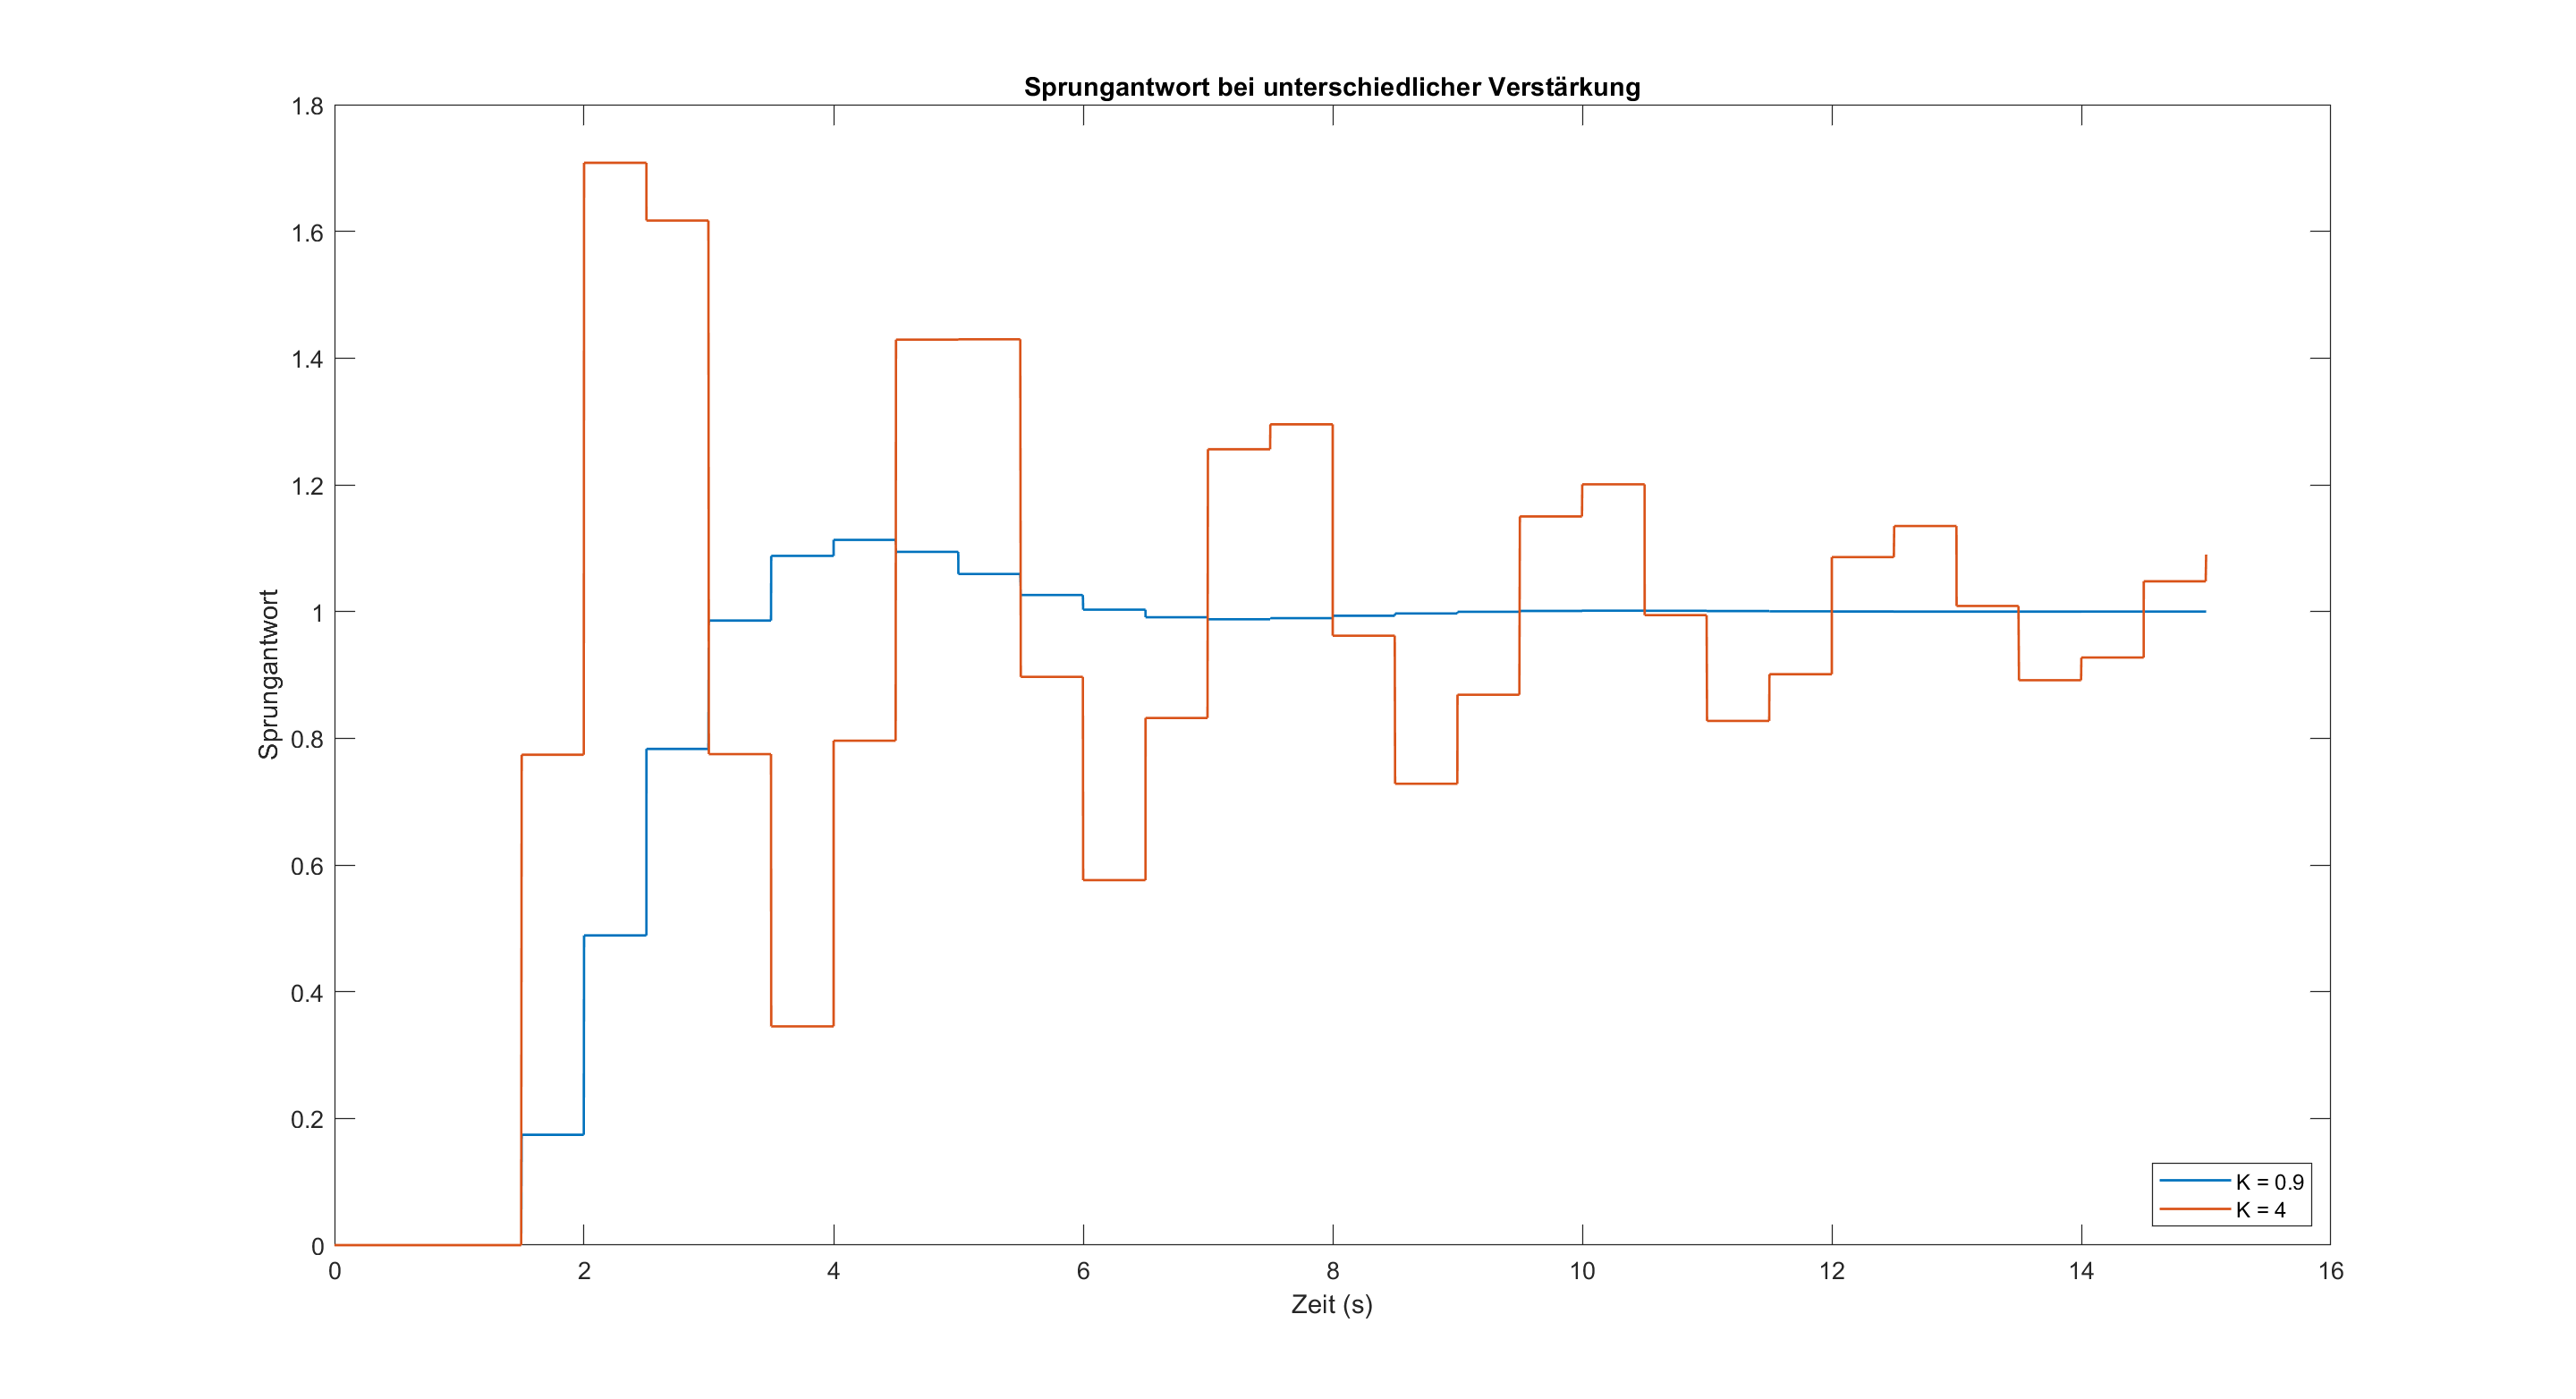
\includegraphics[width=1\linewidth]{images/sprungantworten.png}
	\caption{Sprungantworten bei verschiedenen Reglerverstärkungen}
	\label{sa}
\end{figure}






























    	
    }
    {%
    	%file does not exist
    }




    \label{endOfArabicNumbering}
    \clearpage

    \ifappendix	
        % !TeX root = ../dokumentation.tex
\setpagestylefoot
\renewcommand{\thefigure}{A\arabic{figure}}
\renewcommand\thelstlisting{A\arabic{lstlisting}}
\renewcommand\thetable{A\arabic{table}}

% Nummer des Inhaltes mit \setcounter{figure}{"`Number"'} (figure, lstlisting or table) ändern wenn nötig



% Quellenverzeichnis nach Literatur und Weblinks trennen
%\printbibliography[heading=subbibintoc,title={Literatur},nottype=online]
%\printbibliography[heading=subbibintoc,title={Weblinks},type=online]

% Quellenverzeichnis nicht trennen
\ifliteratur
    \printbibliography
\fi

%\addchap{\langanhang}

% Glossar
\ifglossar
    \printglossary[style=altlist,title=\langglossar]
\fi

    \fi
\end{document}
